%      % GPRS
\subsection{General Packet Radio Service --- GPRS}%
\label{sec:gprs}
\gls{gprs} is a packet based wireless communication service that offers data
rates from 9.05 up to 171.2 Kbps and continuous connection to the Internet for
mobile phone and computer users~\cite{sanders2003gprs}.
GPRS is based on \gls{gsm} communications and complements existing services such
as circuit switched cellular phone connections and the \gls{sms}.
However, \gls{gprs} is packet oriented (like the Internet), enabling packet data
to be sent to or from a mobile device, closing many of the gaps in the \gls{gsm}
standard, namely~\cite{sanders2003gprs}:
\begin{itemize}
\item enable access to company \gls{lan} and the Internet;
\item provide reasonably high data transmission rates;
\item enable the subscriber to be reachable at all times --- not only for
  telephone calls but also for information such as new emails or latest news:
\item offer flexible access, either for many subscribers at low data rates or
  few subscribers at high data rates, optimizing network usage;
\item offer low cost access to new services
\end{itemize}
A \gls{gsm} network is not able to transmit data in packet switched mode, as
required by \gls{gprs}. Thus, two additional modules were required: \gls{sgsn}
and \gls{ggsn}, yielding the \gls{gsm}/\gls{gprs} network depicted in Fig.~\ref{fig:gprs-network}.
On the user side there is a mobile device known as the \gls{ms}, consisting of a
\gls{me} and the \gls{sim}. For \gls{gprs}, the \gls{me} needs to be equipped
with packet transmission capabilities, constituting three different classes of
\gls{gprs} equipment~\cite{sanders2003gprs}:
\begin{itemize}
\item Class A:~equipment that can handle voice calls and packet data transfers
  at the same time;
\item Class B:~equipment that can handle voice or packet data traffic (but not
  simultaneously) and can put a packet transfer on hold to receive a phone call;
\item Class C:~equipment that can handle both voice and data, but has to
  disconnect from one mode explicitly in order to enable the other.
\end{itemize}
% GPRS network
\begin{figure}[!hbt]
\centering
    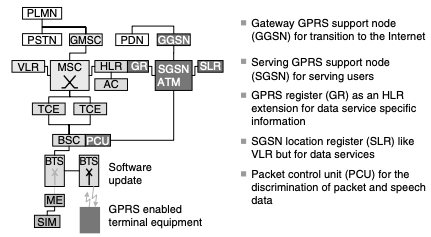
\includegraphics[width=0.5\textwidth]{./img/gprs-network.png}
  \caption{GSM/GPRS network (withdrawn from~\cite{sanders2003gprs})}%
\label{fig:gprs-network}
\end{figure}

The predominant protocol in the world of data networks is the \gls{ip}, enabling
the networking of different network architectures and the standardization of
applications. In the mobile network \gls{gprs} the subscriber has a logical
\gls{ip} connection with an external data network, representing an actual member
of this \gls{ip} network. Packets can then be transferred between the \gls{ms}
and a server in the \gls{ip} network, with the \gls{gprs} standard describing
how they are transmitted on the radio interface and through the whole \gls{gprs}
network.

Prior to the data transfer three important procedures must be
performed~\cite{sanders2003gprs} (see Fig.~\ref{fig:gprs-procedures}):
\begin{enumerate}
\item \uline{gls{gprs} Attach}: the \gls{ms} must be attached in the GPRS network. This is a logical procedure between the \gls{ms} and the \gls{sgsn}
  which takes note of the position, i.e.~the `routing area', of the \gls{ms}. Storing and updating the position of the \gls{ms} is particularly
  important for \gls{dl} transmissions because this information enables the \gls{gprs}
  network to locate the \gls{ms}.
\item \uline{Activation of a \gls{pdp} context}: A
  connection between the \gls{ms} and the \gls{ggsn} must be set up, so each
  node in the GPRS network knows how it has to forward the IP packets of this
  \gls{ms}.
\item \uline{Data transfer}: the path between the MS and the external data network is
  prepared, so IP packets can be sent through the GPRS network towards the
  destination address.
\end{enumerate}
% GPRS network
\begin{figure}[!hbt]
\centering
    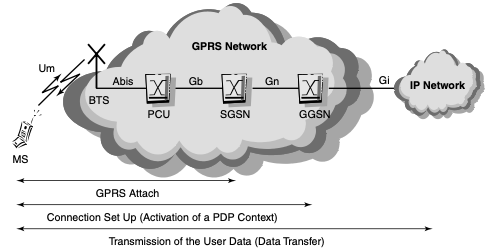
\includegraphics[width=0.7\textwidth]{./img/gprs-procedures.png}
  \caption{GPRS procedures (withdrawn from~\cite{sanders2003gprs})}%
\label{fig:gprs-procedures}
\end{figure}

Thus, the user required hardware for implementation of a GSM/GPRS network is the
\gls{me}, namely, a GSM/GPRS modem and a \gls{sim} card with subscription to a
mobile operator. A GSM/GPRS modem is generally driven through the RS-232 bus,
using the Hayes command set (\gls{at} commands) to interface it.
%%% Local Variables:
%%% mode: latex
%%% TeX-master: "../../../dissertation"
%%% End:
